\documentclass[11pt]{article}
\newcommand{\shorttitle}{Topic 2: Reinforcement learning}
\usepackage[T1]{fontenc}
\usepackage[utf8]{inputenc}
\usepackage{lmodern}
\usepackage[a4paper,margin=23mm,headheight=15pt]{geometry}
\usepackage{amsmath,amssymb,bm,graphicx,booktabs,longtable,array}
\usepackage{xcolor,microtype,enumitem,fancyhdr,fancyvrb,titlesec,tikz}
\usepackage[breakable]{tcolorbox}
\usepackage{hyperref}
\definecolor{navy}{HTML}{163653}
\definecolor{teal}{HTML}{007F86}
\definecolor{pale}{HTML}{EEF5F7}
\hypersetup{colorlinks=true,linkcolor=navy,urlcolor=teal,pdfauthor={Study notes based on the supplied teacher slides}}
\pagestyle{fancy}\fancyhf{}
\fancyhead[L]{\small\sffamily\color{navy}Artificial Intelligence}
\fancyhead[R]{\small\sffamily\color{navy}\shorttitle}
\fancyfoot[C]{\small\thepage}
\renewcommand{\headrulewidth}{0.3pt}
\titleformat{\section}{\Large\sffamily\bfseries\color{navy}}{\thesection}{0.7em}{}
\titleformat{\subsection}{\large\sffamily\bfseries\color{teal}}{\thesubsection}{0.6em}{}
\titleformat{\subsubsection}{\normalsize\sffamily\bfseries\color{navy}}{\thesubsubsection}{0.6em}{}
\setcounter{tocdepth}{2}\setcounter{secnumdepth}{2}
\setlength{\parindent}{0pt}\setlength{\parskip}{6pt plus 1pt}
\linespread{1.06}\setlist{itemsep=3pt,topsep=4pt,leftmargin=1.5em}
\setlength{\emergencystretch}{3em}
\newtcolorbox{keyidea}[1]{breakable,colback=pale,colframe=teal,boxrule=0.6pt,arc=1mm,title={#1},fonttitle=\sffamily\bfseries,coltitle=white,colbacktitle=teal}
\newtcolorbox{careful}[1]{breakable,colback=white,colframe=navy,boxrule=0.6pt,arc=1mm,title={#1},fonttitle=\sffamily\bfseries,coltitle=navy,colbacktitle=pale}
\newcommand{\sources}[1]{{\small\color{teal}\textit{Teacher slides: #1}}\par\nopagebreak[4]}
\newcommand{\newsection}[1]{\par\begingroup\skip0=\pagegoal\advance\skip0 by-\pagetotal\ifdim\skip0<12\baselineskip\newpage\fi\endgroup\section{#1}}
\newcolumntype{P}[1]{>{\raggedright\arraybackslash}p{#1}}
\newcommand{\E}{\operatorname{E}}
\newcommand{\Var}{\operatorname{Var}}
\newcommand{\Cov}{\operatorname{Cov}}
\newcommand{\R}{\mathbb{R}}
\newcommand{\argmax}{\operatorname*{arg\,max}}
\newcommand{\argmin}{\operatorname*{arg\,min}}
\newcommand{\relu}{\operatorname{ReLU}}
\newcommand{\codeinline}[1]{\texttt{\detokenize{#1}}}
\DefineVerbatimEnvironment{code}{Verbatim}{fontsize=\small,samepage=true,frame=single,rulecolor=\color{teal},framesep=2.5mm}
\newcommand{\cover}[3]{%
\begin{titlepage}\vspace*{12mm}
{\sffamily\color{teal}\large ARTIFICIAL INTELLIGENCE\par}\vspace{9mm}
{\sffamily\bfseries\color{navy}\Huge TOPIC #1\par}\vspace{5mm}
{\sffamily\color{navy}\LARGE #2\par}\vspace{11mm}
{\large Explanatory study notes\par}
{\large Theory, worked examples and revision questions\par}\vspace{12mm}
\begin{keyidea}{What you should be able to do}#3\end{keyidea}
\vfill
Based on the teacher PDFs supplied in \texttt{Lecture Slides}. The notes explain and reorganize that material. Worked calculations are study examples derived from the slide concepts, unless explicitly identified as a slide exercise. Clarifications of ambiguous or incorrect expressions are marked in context. References use \textbf{PDF page numbers}, counted from 1, rather than printed slide numbers.
\par\vspace{4mm}{\small English edition\enspace\textbullet\enspace 2 October 2026}
\end{titlepage}\setcounter{page}{2}}

\hypersetup{pdftitle={Topic 2 - Reinforcement Learning, MDPs, Q-Learning and Policy Search}}
\begin{document}
\cover{2}{Reinforcement learning, MDPs and policy search}{Formulate a sequential task as an MDP; derive Bellman updates; distinguish planning, Monte Carlo and TD learning; calculate SARSA and Q-learning updates; explain feature approximation, REINFORCE and actor--critic.}
\tableofcontents\clearpage
\newsection{The central difference: actions change future data}
\sources{2.1. Introduction to Reinforcement Learning, pp. 3--16.}
In supervised learning, a dataset supplies target outputs. In RL, an agent chooses an action, receives a reward and moves to a new state. The action influences both future reward and the experiences from which the agent can learn. A locally good action can lead to poor long-term outcomes.

Use $S_t$ for state, $A_t$ for action and $R_{t+1}$ for the reward received after that action. The slides often use $x_t,a_t$; they represent the same objects. The policy specifies behavior; a value function predicts future reward; a model describes transitions and rewards.
\begin{center}
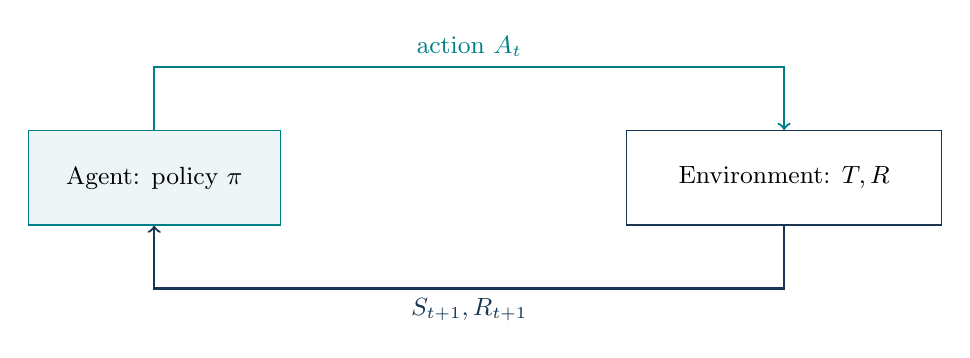
\begin{tikzpicture}[every node/.style={font=\small}]
\node[draw=teal,fill=pale,minimum width=32mm,minimum height=12mm] (a) at (0,0) {Agent: policy $\pi$};
\node[draw=navy,minimum width=40mm,minimum height=12mm] (e) at (8,0) {Environment: $T,R$};
\draw[->,thick,teal] (a.north) -- +(0,0.8) -| node[pos=.25,above] {action $A_t$} (e.north);
\draw[->,thick,navy] (e.south) -- +(0,-0.8) -| node[pos=.25,below] {$S_{t+1},R_{t+1}$} (a.south);
\end{tikzpicture}
\end{center}
The reward hypothesis expresses the objective as expected cumulative scalar reward. Maximizing reward is equivalent to minimizing cost when reward is negative cost. Reward design matters: a large reward for speed and too small a collision penalty can produce unwanted behavior even if learning works correctly.
\subsection{Planning and learning}
Planning uses a known transition/reward model to compute behavior. RL estimates useful quantities from experience when the model is unknown or incomplete. Model-based RL learns a model and then plans; model-free RL learns values or policies directly. ``Model-free'' means an explicit transition model is unnecessary, not that the agent has no learned representation.
\newsection{Markov decision processes}
\sources{2.1. Introduction to Reinforcement Learning, pp. 7--13; 2.2. Markov decision processes, pp. 2--6.}
An MDP consists of a state space $\mathcal S$, action space $\mathcal A$, transition probabilities $T(s,a,s')=P(S_{t+1}=s'\mid S_t=s,A_t=a)$ and reward function $R(s,a,s')$. We also specify a discount factor, a start distribution and terminal conditions where relevant.

The controlled Markov property is
\[
P(S_{t+1},R_{t+1}\mid S_t,A_t,\text{earlier history})
=P(S_{t+1},R_{t+1}\mid S_t,A_t).
\]
State must summarize the history relevant for future prediction. Current position alone may be insufficient for racing if velocity affects the next position. A stationary policy depends only on state; finite-horizon policies may also need the remaining time.

A deterministic policy chooses $a=\pi(s)$. A stochastic policy gives probabilities $\pi(a\mid s)$ summing to one. Under a fixed policy, transition probabilities can be averaged over actions to form a Markov chain on states.
\subsection{Gridworld and partial observability}
The gridworld slides give four directional actions and noisy motion: a chosen north move succeeds with probability $0.8$ and slips sideways with probability $0.1$ each. Hitting a wall can leave the agent in place. Several outcomes reaching the same state must have their probabilities added.

If the agent observes only an imperfect signal of the state, the problem is partially observable. A belief distribution over hidden states can act as a sufficient state representation. The supplied notes introduce this idea but subsequent derivations assume fully observed MDP states.
\newsection{Returns, discounting and terminal states}
\sources{2.2. Markov decision processes, pp. 7--11.}
Define return
\[
G_t=\sum_{k=0}^{\infty}\gamma^kR_{t+k+1}
=R_{t+1}+\gamma G_{t+1}.
\]
For an episode ending at time $T$, stop the sum at the final transition and set the terminal state's remaining return to zero. The reward \emph{for entering} the terminal state is still included.

$\gamma=0$ considers only the next reward; $\gamma$ close to one values distant reward more strongly. For bounded rewards and $0\leq\gamma<1$, the infinite sum is bounded by $R_{\max}/(1-\gamma)$ in absolute value. Undiscounted episodic returns can be well defined, but merely having a terminal state does not ensure every policy reaches it in a suitably finite expected time.
\subsection{Worked discounting comparison}
Action L reaches reward 10 after three transitions with no earlier reward. Action R reaches reward 1 after one transition. At the initial state,
\[
G_L=10\gamma^2,\qquad G_R=1.
\]
They are equal at $\gamma=1/\sqrt{10}\approx0.316$. For $\gamma=0.1$, prefer R; for $\gamma=0.9$, prefer L. This illustrates the teacher's left-versus-right quiz, with the reward timing explicitly stated so that the exponent is unambiguous.
\newsection{Value functions and Bellman expectation equations}
\sources{2.2. Markov decision processes, pp. 11--15.}
\[
V^\pi(s)=\E_\pi[G_t\mid S_t=s],\qquad
Q^\pi(s,a)=\E_\pi[G_t\mid S_t=s,A_t=a].
\]
$V^\pi$ averages over the first action prescribed by the policy. $Q^\pi$ fixes that action, then follows $\pi$. A value is not the immediate reward: it includes discounted continuation.

Expand $G_t=R_{t+1}+\gamma G_{t+1}$ and average over next states:
\[
Q^\pi(s,a)=\sum_{s'}T(s,a,s')\big[R(s,a,s')+\gamma V^\pi(s')\big].
\]
Then average over policy actions:
\begin{align*}
V^\pi(s)&=\sum_a\pi(a\mid s)Q^\pi(s,a),\\
V^\pi(s)&=\sum_a\pi(a\mid s)\sum_{s'}T(s,a,s')
[R(s,a,s')+\gamma V^\pi(s')].
\end{align*}
For small finite MDPs, this is a linear system $V^\pi=r^\pi+\gamma P^\pi V^\pi$. Solve $(I-\gamma P^\pi)V^\pi=r^\pi$, or repeatedly apply the expected update.
\subsection{Worked policy evaluation}
Under a fixed policy, state A always moves to B with reward 1; B always moves to terminal with reward 2. With $\gamma=0.9$,
\[
V(B)=2,\qquad V(A)=1+0.9(2)=2.8.
\]
Starting all values at zero, synchronous evaluation gives $(V_1(A),V_1(B))=(1,2)$, followed by $(2.8,2)$. Information propagates backward one transition per sweep.
\newsection{Optimality and dynamic programming}
\sources{2.2. Markov decision processes, pp. 16--24.}
\subsection{Replace a policy average with the best action}
For the finite discounted setting considered in the slides,
\[
V^*(s)=\max_\pi V^\pi(s),\qquad Q^*(s,a)=\max_\pi Q^\pi(s,a).
\]
Bellman optimality is
\begin{align*}
V^*(s)&=\max_a\sum_{s'}T(s,a,s')[R(s,a,s')+\gamma V^*(s')],\\
Q^*(s,a)&=\sum_{s'}T(s,a,s')[R(s,a,s')+\gamma\max_bQ^*(s',b)].
\end{align*}
An optimal policy chooses an action maximizing $Q^*$. Randomizing among equally good actions also preserves optimal value. Extracting a greedy policy from $V$ requires the transition and reward model; extracting it from $Q$ requires only an action maximization.
\subsection{Three different algorithms}
\begin{longtable}{@{}P{.23\textwidth}P{.34\textwidth}P{.34\textwidth}@{}}
\toprule Algorithm & Update & Purpose\\\midrule\endhead
Policy evaluation & Expected backup under fixed $\pi$ & Predict that policy's value.\\
Value iteration & Maximum expected backup & Approach optimal value directly.\\
Policy iteration & Evaluate policy, then improve greedily & Alternate prediction and improvement.\\\bottomrule
\end{longtable}
For synchronous value iteration, compute every $V_{k+1}(s)$ from the old $V_k$ table, then replace the table. In-place updates instead use some newly computed values in the same sweep. Both can be useful, but they give different intermediate iterates.

With $\gamma<1$, the Bellman operator contracts differences in the maximum norm, explaining convergence of repeated backups. A small update difference is a stopping diagnostic; an exact optimal-value claim would require accounting for the residual and discount factor.
\subsection{Worked stochastic backup}
Action a yields reward 2 and successor value 5 with probability $0.8$, or reward $-1$ and successor value 1 with probability $0.2$. For $\gamma=0.9$,
\[
Q(s,a)=0.8(2+0.9\cdot5)+0.2(-1+0.9\cdot1)=5.18.
\]
This is a full expected backup. RL sample updates approximate such averages using realized transitions.
\newsection{Monte Carlo: learn from complete returns}
\sources{2.3. Q-learning, pp. 6--17.}
For policy evaluation, follow $\pi$, collect complete episodes, calculate the return from each visited state and average those returns. This does not require an explicit model of the environment.

The incremental mean after $N(s)$ samples is
\[
V(s)\leftarrow V(s)+\frac1{N(s)}[G_t-V(s)].
\]
Replacing $1/N(s)$ with constant $\alpha$ gives an exponentially weighted estimate that discounts older samples. This can track change but generally leaves sampling fluctuations.

First-visit MC uses only the first occurrence of a state in each episode; every-visit MC uses every occurrence. Both wait for the episode's rewards to be known. MC does not bootstrap from current value estimates, but complete returns can have high variance and cannot be formed directly for never-ending episodes without another strategy.
\subsection{Worked incremental average}
Returns from a state are $3,5,1$. Starting at zero with $\alpha_N=1/N$, estimates become $3$, $4$, then $4+(1/3)(1-4)=3$. This is exactly the sample average of the three returns.
\newsection{Temporal difference: update before the episode ends}
\sources{2.3. Q-learning, pp. 18--26.}
TD(0) uses one observed reward plus estimated successor value:
\[
\delta_t=R_{t+1}+\gamma V(S_{t+1})-V(S_t),\qquad
V(S_t)\leftarrow V(S_t)+\alpha\delta_t.
\]
The quantity $\delta_t$ is the TD error. Positive error means the observed transition looked better than predicted. \textbf{Bootstrapping} means that the target uses another current estimate.
\begin{longtable}{@{}P{.18\textwidth}P{.39\textwidth}P{.34\textwidth}@{}}
\toprule Method & Target & Main distinction\\\midrule\endhead
Dynamic programming & Expected $R+\gamma V(S')$ & Needs a model; averages successors.\\
Monte Carlo & Observed complete $G_t$ & Samples experience; no bootstrap.\\
TD(0) & Observed $R+\gamma V(S')$ & Samples experience; bootstraps.\\\bottomrule
\end{longtable}
TD can learn from incomplete episodes and continuing tasks. It exploits Markov structure and often has lower target variance than MC, while its target can initially be biased by inaccurate successor estimates. Convergence statements require assumptions about visitation, learning rates and representation; unlimited experience alone does not guarantee stability for every approximation.
\subsection{Worked TD update}
Let $V(s)=4$, $V(s')=5$, reward $2$, $\gamma=0.9$ and $\alpha=0.1$. The target is $6.5$, error is $2.5$ and new value is $4.25$. If $s'$ is terminal, continuation is zero, so the target is only $2$ and new value is $3.8$.

$\gamma$ controls preference for future rewards. $\alpha$ controls how rapidly estimates change. They have different roles even though both commonly lie between zero and one. TD($\lambda$), named in the slides, combines information across multiple steps; no detailed eligibility-trace derivation is supplied.
\newsection{Exploration, exploitation and regret}
\sources{2.3. Q-learning, pp. 27--33.}
Exploitation chooses the currently best estimated action. Exploration tests uncertain alternatives. Acting greedily from inaccurate estimates can prevent the agent from discovering a better action; acting randomly forever can waste reward after good choices become known.

An $\epsilon$-greedy policy selects a random legal action with probability $\epsilon$ and a greedy legal action otherwise. If random selection includes the greedy action and there are $m$ actions, its probability is $1-\epsilon+\epsilon/m$ when the maximizer is unique. Break maximizing ties without an arbitrary systematic preference.

Optimistic initialization gives unknown actions attractive initial values. Upper-confidence ideas add a bonus for uncertainty. Regret compares expected reward accumulated by the learner with an appropriate optimal benchmark; it measures the cost of learning as well as eventual behavior.
\begin{careful}{Qualifications to the exploration slide}
The random-policy limit on p. 32 is exploration. Random behavior does not itself constitute an optimal learned policy, and visiting every action is not guaranteed without reachability and sampling assumptions. Exploration must be adequate for the problem; a small fixed $\epsilon$ is not a universal convergence recipe.
\end{careful}
\newsection{SARSA and Q-learning}
\sources{2.3. Q-learning, pp. 28--38.}
\subsection{On-policy SARSA}
The name refers to $(S_t,A_t,R_{t+1},S_{t+1},A_{t+1})$. Select the next action under the same behavior policy and update
\[
Q(S_t,A_t)\leftarrow Q(S_t,A_t)+\alpha
[R_{t+1}+\gamma Q(S_{t+1},A_{t+1})-Q(S_t,A_t)].
\]
The target includes the effects of the policy's actual exploration. This can make it value safer behavior when exploratory mistakes have a high cost.
\subsection{Off-policy Q-learning}
Q-learning uses the best estimated successor action:
\[
Q(S_t,A_t)\leftarrow Q(S_t,A_t)+\alpha
[R_{t+1}+\gamma\max_aQ(S_{t+1},a)-Q(S_t,A_t)].
\]
The behavior policy can be exploratory, but the target policy is greedy. That difference makes it off-policy. Q-learning does not need to sample a second action to calculate its target; it takes a maximum over available values. This clarifies the shorthand on p. 37.
\subsection{Worked comparison from one transition}
Suppose current $Q(s,a)=4$, reward is $1$, and successor values are $[2,6]$. Exploration actually selects the action with value $2$. With $\gamma=0.9$, $\alpha=0.2$:
\begin{align*}
\text{SARSA target}&=1+0.9(2)=2.8,&Q_{\mathrm{new}}&=3.76,\\
\text{Q-learning target}&=1+0.9(6)=6.4,&Q_{\mathrm{new}}&=4.48.
\end{align*}
Both updates use the same observed reward and transition; they differ in assumed future behavior.
\subsection{Algorithm and convergence scope}
Initialize values, including zero continuation at terminal states. Repeatedly choose an exploratory legal action, observe the transition, calculate the target, update the visited pair, and move to the successor. Stop at termination.

Tabular discounted Q-learning has convergence results when all relevant state--action pairs are visited sufficiently and per-pair step sizes satisfy conditions such as $\sum_t\alpha_t=\infty$, $\sum_t\alpha_t^2<\infty$. Constant step sizes, changing environments and function approximation need separate consideration.
\newsection{Approximate Q-learning and the Pacman connection}
\sources{2.3. Q-learning, pp. 39--47.}
\subsection{A small weight vector replaces a large table}
Represent a state--action pair by features $f_i(s,a)$, such as distance to food, proximity to a ghost and a bias feature:
\[
Q_w(s,a)=\sum_iw_if_i(s,a)=w^Tf(s,a).
\]
One experience can change predictions for many pairs sharing features. This generalization is also a limitation: states with equal features receive equal predictions even when the omitted information matters.

Define the target and TD error
\[
y=r+\gamma\max_bQ_w(s',b),\qquad\delta=y-Q_w(s,a).
\]
The linear update is
\[
\boxed{w_i\leftarrow w_i+\alpha\delta f_i(s,a)}.
\]
It is a \textbf{semi-gradient} step: treat the target as fixed while differentiating the current prediction. Differentiating the same weights through the bootstrap target produces a different algorithm.
\subsection{Worked slide Pacman calculation}
On p. 45, weights for food and ghost features start at $4,-1$, with feature values $0.5,1$. Thus $Q=4(0.5)-1(1)=1$. Reward is $-500$, successor continuation is zero and $\alpha=0.004$:
\[
\delta=-501,\quad
w_{\mathrm{food}}=4+0.004(-501)(0.5)=2.998,
\]
\[
w_{\mathrm{ghost}}=-1+0.004(-501)(1)=-3.004.
\]
The slides round the updated weights to $3,-3$. The new estimate on the same features is approximately $-1.505$.
\subsection{How the formulas map to the lab agent}
Without changing lab code, use this conceptual map when reading \codeinline{qlearningAgents.py}:
\begin{itemize}
\item A Q lookup supplies the stored table value or the feature-weight dot product.
\item State value is the maximum Q among legal actions; a terminal state has zero continuation.
\item Policy extraction returns a maximizing legal action; behavior adds $\epsilon$-greedy exploration.
\item An observed transition updates one table entry or the active feature weights using the same TD error.
\end{itemize}
For all feature-weight updates from one transition, calculate a single TD error from the pre-update prediction. Recomputing it after every individual weight change would alter the intended update.
\subsection{The deadly triad}
The slides call attention to the combination of function approximation, bootstrapping and off-policy learning. Together they can cause instability or divergence. The usual name is \textbf{deadly triad}, rather than ``Deadline triad.'' Removing one component avoids this particular combination, but does not automatically guarantee convergence for every algorithm or nonlinear model.
\newsection{Policy search: learn action probabilities directly}
\sources{2.4. Policy Search, pp. 2--11.}
Parameterize $\pi_\theta(a\mid s)$ and maximize expected return. Policy methods can represent stochastic choices naturally and are useful for continuous actions, where a discrete maximization over Q-values may be difficult. Their sampled gradients can have high variance and their objectives are usually nonconvex.
\subsection{Trajectory probability and the log-derivative identity}
For an episode $\tau$ of $T$ transitions,
\[
p_\theta(\tau)=p(s_0)\prod_{t=0}^{T-1}
\pi_\theta(a_t\mid s_t)T(s_t,a_t,s_{t+1}).
\]
If environment dynamics do not depend on policy parameters, their log derivatives vanish. Using $\nabla p=p\nabla\log p$,
\[
\nabla_\theta J=\E\!\left[G_0\sum_t\nabla_\theta\log\pi_\theta(A_t\mid S_t)\right].
\]
For the slides' undiscounted episodic setting, causality allows replacing the full return beside each score gradient by the return from that step onward:
\[
\nabla_\theta J=\E\!\left[\sum_tG_t\nabla_\theta\log\pi_\theta(A_t\mid S_t)\right].
\]
An action cannot influence rewards that have already occurred. The environment need not be differentiable for this likelihood-ratio estimator. Discounted objectives require consistent return and time-weight conventions; the teacher derivation uses $\gamma=1$.
\subsection{Softmax policy}
For scores $z_a=\theta^Tf(s,a)$,
\[
\pi_\theta(a\mid s)=\frac{e^{z_a}}{\sum_be^{z_b}},\qquad
\nabla_\theta\log\pi_\theta(a\mid s)
=f(s,a)-\sum_b\pi_\theta(b\mid s)f(s,b).
\]
The gradient compares the chosen action's features to their policy-weighted average. Multiplying by positive return increases its relative tendency; a negative return does the opposite.
\newsection{REINFORCE and actor--critic}
\sources{2.4. Policy Search, pp. 12--19.}
\subsection{REINFORCE}
Generate an episode under the current policy, calculate returns backward, and ascend a sampled policy gradient:
\[
\theta\leftarrow\theta+\eta\sum_tG_t\nabla_\theta\log\pi_\theta(A_t\mid S_t).
\]
Collect episode quantities under the same policy before applying the update. With a minimization-based optimizer, use the negative surrogate loss
\[
L(\theta)=-\sum_tG_t\log\pi_\theta(a_t\mid s_t).
\]
Treat sampled returns as constants for this score-function gradient. Automatic differentiation computes the policy derivative; it does not magically differentiate the environment or calculate returns.

An action-independent baseline $b(s_t)$ can replace $G_t$ with $G_t-b(s_t)$ without changing the expected gradient, since $\sum_a\pi(a\mid s)\nabla\log\pi(a\mid s)=0$. This is a useful explanation of variance reduction when connecting REINFORCE to a learned critic.
\subsection{Worked two-action policy update}
Let $\pi(a_1)=\sigma(\theta)$, initially $\theta=0$, so both actions have probability $0.5$. If $a_1$ is sampled and return is 4, then $\partial_\theta\log\pi(a_1)=1-0.5=0.5$. With $\eta=0.1$, the update is $\theta=0.2$, giving $\pi(a_1)\approx0.550$. Positive return makes that action more likely.
\subsection{The actor and critic have different jobs}
The actor updates policy parameters $\theta$. The critic updates value parameters $w$. The slide algorithm uses a Q critic and an on-policy TD target:
\begin{align*}
\theta&\leftarrow\theta+\eta_\theta\nabla_\theta\log\pi_\theta(a_t\mid s_t)Q_w(s_t,a_t),\\
\delta&=r_{t+1}+\gamma Q_w(s_{t+1},a_{t+1})-Q_w(s_t,a_t),\\
w&\leftarrow w+\eta_w\delta f(s_t,a_t).
\end{align*}
The critic replaces a noisy full return with an estimate, often reducing variance while introducing approximation bias. A related value-critic formulation uses $r+\gamma V(s')-V(s)$ as an advantage estimate; it is useful to recognize the relation without confusing it with the specific Q-based slide algorithm.

The slides also mention hill climbing, evolutionary algorithms and Bayesian optimization. They offer alternatives when gradients are unavailable or less suitable. Their ability to explore broadly does not guarantee an exact global optimum within a finite evaluation budget. These names are introductions; no further algorithmic derivation is supplied here.
\newsection{Revision questions and answers}
\subsection{Questions}
\begin{enumerate}
\item What information must an MDP state contain?
\item What is the difference between reward and value?
\item Why can you extract a greedy policy from Q without a transition model?
\item Which of DP, MC and TD bootstrap? Which require a model?
\item Why does Q-learning remain off-policy when behavior is $\epsilon$-greedy?
\item For $Q=2$, reward $3$, terminal successor and $\alpha=0.5$, what is new Q?
\item Can a large Q table generalize automatically to an unseen state?
\item Why are approximate Q-learning updates called semi-gradients?
\item Why is REINFORCE implemented with a negative weighted log probability?
\item Which three ingredients make up the deadly triad?
\end{enumerate}
\subsection{Answers}
\begin{enumerate}
\item Enough to make future transition/reward distributions independent of earlier history, given the action.
\item Reward is one step's feedback; value is expected future cumulative reward.
\item Q already evaluates each possible first action; only maximization is needed.
\item DP and TD bootstrap. Standard MC does not. DP requires the model.
\item The target assumes greedy continuation, different from exploratory behavior.
\item $2+0.5(3-2)=2.5$; terminal continuation is zero.
\item No. Features or another approximation supply generalization.
\item They differentiate the current prediction while keeping the bootstrap target fixed.
\item Minimizing that surrogate performs sampled gradient ascent on return.
\item Function approximation, bootstrapping and off-policy learning.
\end{enumerate}
\newsection{Source guide}
\texttt{2.1. Introduction to Reinforcement Learning.pdf}: reward, policy, model and sequential interaction. \texttt{2.2. Markov decision processes.pdf}: returns, Bellman equations and planning. \texttt{2.3. Q-learning.pdf}: MC, TD, exploration, SARSA, Q-learning and feature approximation. \texttt{2.4. Policy Search.pdf}: trajectory gradients, REINFORCE, actor--critic and optimization alternatives. The Pacman numerical update is worked from p. 45 of the Q-learning deck. The lab connection explains those slide formulas without using lab code as an additional theory source.
\end{document}
